\documentclass[preprint,12pt]{elsarticle}

\usepackage{hyperref}
\usepackage{graphicx}
\usepackage{subcaption}
\usepackage{amssymb}
\usepackage{amsmath}
\usepackage{multirow}
\usepackage{relsize}
\usepackage[utf8]{inputenc}
\usepackage{cleveref}
\usepackage{algorithm}
\usepackage[noend]{algpseudocode}
\usepackage[section]{placeins}
\usepackage{booktabs}
\usepackage{physics}
\usepackage{breqn}

% For the TODOs
\usepackage{xcolor}
\usepackage{xargs}
\usepackage[colorinlistoftodos,textsize=footnotesize]{todonotes}
\newcommand{\todoin}{\todo[inline]}
% from here: https://tex.stackexchange.com/questions/9796/how-to-add-todo-notes
\newcommandx{\unsure}[2][1=]{\todo[linecolor=red,backgroundcolor=red!25,bordercolor=red,#1]{#2}}
\newcommandx{\change}[2][1=]{\todo[linecolor=blue,backgroundcolor=blue!25,bordercolor=blue,#1]{#2}}
\newcommandx{\info}[2][1=]{\todo[linecolor=OliveGreen,backgroundcolor=OliveGreen!25,bordercolor=OliveGreen,#1]{#2}}

%Boldtype for greek symbols
\newcommand{\teng}[1]{\ensuremath{\boldsymbol{#1}}}
\newcommand{\ten}[1]{\ensuremath{\mathbf{#1}}}

\usepackage{lineno}

\journal{}

\begin{document}

\begin{frontmatter}

  \title{Rigid fluid coupling}
  \author[IITB]{Dinesh Adepu \corref{cor1}}
  \ead{adepu.dinesh.a@gmail.com} \author[IITB]{Prabhu Ramachandran}
  \ead{prabhu@aero.iitb.ac.in} \address[IITB]{Department of Aerospace
    Engineering, Indian Institute of Technology Bombay, Powai, Mumbai 400076}

\cortext[cor1]{Corresponding author}

\begin{abstract}
  In this paper, a particle-based framework is developed to study the
  transport of rigid bodies in fluid flows. The interaction between the rigid
  bodies is handled with the discrete element method (DEM), where a new
  contact force model is used to handle the arbitrarily shaped rigid bodies.
  The fluid phase is modeled using a variant of the weakly compressible
  smoothed particle hydrodynamics (SPH) scheme, corrected transport velocity
  formulation (CTVF). CTVF provides homogeneous particle distributions and
  smooth pressure variations. The interaction between the fluid and rigid
  bodies is modeled using a dummy particle approach. The accuracy of the
  developed method is evaluated via several numerical examples involving
  analytical and experimental results. The rigid-rigid interaction part of the
  solver is validated through the study of rolling and sliding body cases.
  Further, the collapse of a stack of cylinders under gravity is studied and
  compared against its experimental counterpart. The rigid-fluid interaction
  is studied with the water-entry of different bodies into the hydrostatic
  water tank. As an application, we study the collapse of a stack of cubes due
  to a 3D dam-breaking flow over. The results indicate that the current method
  can effectively model irregular bodies in a fluid flow. Finally, the current
  implementation is made fully open-source and reproducible.
\end{abstract}

\begin{keyword}
%% keywords here, in the form: keyword \sep keyword
{Smoothed particle hydrodynamics}, {Discrete element method}, {Irregular bodies}, {Rigid fluid coupling}

%% MSC codes here, in the form: \MSC code \sep code
%% or \MSC[2008] code \sep code (2000 is the default)

\end{keyword}

\end{frontmatter}

% \linenumbers

\section{Journals in consideration}

Submit to special issue in Water journal.


\section{Introduction}
\label{sec:intro}
Transport of arbitrarily shaped rigid bodies in fluid flows is a common
phenomenon that occurs widely in nature. Debris flowing, the food processing
industry and ice-sea modeling are a few areas to mention. The two-way coupling
between the rigid and the fluid flow is nonlinear and analytical modeling is
not feasible apart from a few simple cases. Mesh-based or meshless schemes are
in practice to study in the numerical setting. *Numerical techniques allow us
to study coupling physics with more flexibility.*

Mesh-based schemes are in practice \cite{dettmer_computational_2006} to model
the fluid while handling rigid-fluid coupling problems. However, these schemes
are unfavorable when dealing with free surface flows and with mediums
undergoing huge deformation \cite{walkley_finite_2005}. Therefore, while
handling RFC problems, meshless methods are preferred in handling the fluid
phase because of their inherent advantage at modeling free surfaces and large
deformations. In meshless techniques, Moving Particle Semi-implicit (MPS) -
Discrete Element Method (DEM) \cite{guo2017numerical} and smoothed particle
hydrodynamics (SPH)-DEM \cite{canelas2016sph} are two among many techniques in
modeling rigid-fluid coupling problems. MPS and SPH are used to model the
fluid phase, while DEM is for rigid body interaction. A coupling strategy is
proposed to handle the interaction between the rigid body and the fluid in
both schemes. In addition to DEM alone to model the rigid-rigid interaction,
there are also works where SPH \cite{amicarelli2015smoothed} itself is used to
model the interaction. But it lacks to incorporate the friction between the
bodies. In the current work we have used SPH to model the fluid dynamics, and
DEM to model the rigid-rigid interaction.

The SPH method is a meshless numerical method initially proposed by
\citet{gingold1977smoothed} and \citet{lucy1977numerical} to model
astrophysics problems and is successful at modeling physics ranging different
fields. \citet{monaghan2005smoothed} provides a detailed review of SPH and its
applications. SPH uses a weakly compressible \cite{adepu2021corrected} or an
incompressible approach \cite{cummins_sph_1999} to model the fluid flow.
Though WCSPH is able to model the fluid flow successfully, it suffers from
high-pressure oscillation and inhomogeneous particle distribution. To overcome
these issues, \cite{PRKP:edac-sph-iccm2015} proposed EDAC and
\cite{marrone_-sph_2011} proposed delta plus where, a diffusion term is added
to the continuity term, while in EDAC a thermodynamically consistent equation
is proposed to evolve the pressure. To get a homogeneous particle
distribution, \cite{acc_stab_xu:jcp:2009} proposed a particle shifting scheme,
where after every iteration particle positions are adjusted such that we reach
a expected level consistency and the particle properties are adjusted to the
new positions using Taylor series expansion. Using the particle shifting
concept , \cite{Adami2013} proposed a transport velocity formulation {TVF} where
the particles are moved with a transport velocity rather than the momentum
velocity to achieve homogeneous particle distribution. Further,
\cite{zhang2017generalized} extended it to handle free surface problems, with
generalized TVF (GTVF). *A transport velocity formulation (\cite{Adami2013})
based scheme, corrected transport velocity formulation (CTVF)
\cite{adepu2021corrected} is used in the current work to model the fluid
dynamics, because of which better particle distribution is achieved leading to
less errors.*

DEM is initially proposed to model the granular soil, bodies in spherical
shape are modeled (DEM paper). Later, rigid bodies with hydrophobic shapes are
handled using different variations of the DEM method. Rigid bodies with
irregular geometries, multi-sphere approach \cite{das2007modeling} This is not
a good approach, one of the reasons is the contact force model is between two
particles, and those particles are assumed as spheres, and the contact
handling is taken care of. This doesn't consider the shape of the surface of
the rigid body in place. SMR-DEM by \citet{zhan2021surface}, dilated
polyhedral DEM \citet{liu_new_2020}, Fourier series-based discrete element
method \citet{lai_fourier_2020}, non-smooth wall modeling by
\citet{amaro_junior_improvement_2019}, GJK-DEM \cite{wachs2012grains3d},
discrete function representation based DEM \cite{lu2012critical}, level set
DEM method \cite{duriez2021precision} are few more. However, these are
complicated to implement and requires additional information to handle the
contact between the bodies in addition to the particle positions, like
connectivity, and it is difficult for 3d extension. The rigid bodies have to
be discretized differently to handle the non-smooth boundaries, or we need
connectivity information to identify the body's shape. However, we need to
generate additional particles on the rigid body to handle the interaction with
the fluid. Also, the discretization needed to handle the rigid-rigid
interaction is not enough to handle the rigid fluid interaction with the above
methods of handling fluid flow. We need additional set of particles to handle
the rigid fluid coupling. In the current work we have extended the contact
force model proposed by \citet{mohseni2021particle} to handle three
dimensional problems, we also incorporate the damping model. This contact
force model can handle the interaction between the rigid bodies from the
particle position data alone, the amount of overlap between the bodies is
computed using a SPH method.

The current work combines CTVF with DEM to model two-way rigid-fluid coupling
of arbitrarily shaped rigid bodies in a fluid flow. The fluid phase is handled
using a corrected transport velocity formulation developed by \cite{adepu2021corrected},
which provides smooth pressure distribution with EDAC formulation and
homogeneous particle distribution, resulting in accurate fluid modeling. A
modified DEM method proposed by Mohseni is used to model the rigid-rigid
interaction between the rigid bodies. The inelastic collision is modeled by
introducing an additional damping term in the contact force model. The
interaction between the fluid phase and rigid bodies is handled using the
ghost particle approach \cite{Adami2012}. We explored different rigid fluid
coupling strategies by simulating high density ratio simulations. To validate
the rigid-rigid contact force model, a free and forced sliding of a 3d cube on
a frictional inclined plane and a cylinder rolling on an inclined plane are
simulated. The collapse of a stack of cylinders is modeled and compared
against the experimental results. A 3d cube released inside a fluid tank is
simulated and compared against the experimental results to validate the
two-way rigid-fluid coupling algorithm. Additionally, two cylinders of the
same diameter are allowed to settle inside a tank in series and side-by-side
configuration and compared against the experimental result. A cylinder of
density 500 $kg/m^3$ is allowed to settle in a hydrostatic tank and expected
to submerge till half of its body. A 3D dam breaking water is allowed to
impact a rigid cube placed at a certain distance and is simulated and compared
against the experimental result. All the results are fully automated with the
automan package \cite{automan2018} and made hundred percent reproducible.


\FloatBarrier%
\section{Rigid body dynamics}
\label{sec:rbd}

% The rigid body is discretized into particles with equal spacing each particle
% with mass $m_i$ and density $\rho_i$. Rigid body has a total 6 degrees of
% freedom (DOF), divided into $3$ translational and $3$ rotational.

\subsection{Governing equations}

The equations governing the dynamics of a rigid body are, balance of linear and
angular momentum given by,
\begin{equation}
  \label{eq:balance_linear_mom}
  \frac{d \; (M \ten{v}_{cm})}{d t} = \sum_i \ten{F}_i,
\end{equation}
\begin{equation}
  \label{eq:balance_angular_mom}
  \frac{d \ten{L}}{d t} = \teng{\tau}
\end{equation}
where $\ten{v}_{cm}, \ten{F}_i, \teng{\tau}, \ten{L} $ is the torque about the center of mass
($\ten{x}_{cm}$) due to the forces on the particles,
\begin{equation}
  \label{eq:torque}
  \teng{\tau}_{cm} = \sum_i \ten{F}_i \times (\ten{r}_{cm} - \ten{r}_{i}).
\end{equation}
$\ten{L}$ is the angular momentum of the rigid body about the center of mass,
computed as
\begin{equation}
  \label{eq:moi}
  \teng{L} =
  \sum_i \; \ten{r}_i \times \; (\teng{\omega} \times \ten{r}_i)
  = \sum_i \; m_i \; [(\ten{r} \cdot \ten{r}) \ten{I} - \ten{r} \otimes \ten{r}]
\end{equation}



% \begin{equation}
%   \label{eq:omega_compute}
%   \teng{\omega} = \textit{\teng{I}}^{-1} \; \ten{L}
% \end{equation}


\subsection{State of the rigid body}

The state of the rigid body at a given time ($t$) can described using position
and velocity of the center of mass ($\ten{x}_{cm}$), velocity of center of
mass ($\ten{v}_{cm}$), a rotation matrix ($\ten{R}$) which is used to
determine the orientation of the body axis vectors with respect to global
frame, to define the three rotational degrees of freedom and angular
velocity($\teng{\omega}$). The center of mass is computed with
\begin{equation}
  \label{eq:center_of_mass}
  \ten{x}_{cm} = \frac{\sum_i m_i \; \ten{x}_{i} }{\sum_i m_i }
\end{equation}

\begin{figure}[!htpb]
  \centering
  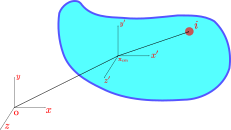
\includegraphics[width=0.5\textwidth]{images/rigid_body/rigid_body}
  \caption{Body frame and local frame description of rigid body}
  \label{fig:gloabl_body_frame_rb}
\end{figure}
The position of the discretized particle ($P$) in
\cref{fig:gloabl_body_frame_rb} belonging to the rigid body at time $t$ can be
computed.
\begin{equation}
  \label{eq:rb_particle_pos_update}
  \ten{r}_i = \ten{R} \cdot \overline{\ten{r}}_{i}
\end{equation}
Here $\overline{\ten{r}}_{i}$ is the position of the particle $i$ about the
body frame axis and remains constant. The rotation matrix $R$ is used to bring
the body frame axis position vector to the global frame axis $\ten{O}$, to
compute the position vector about the global frame axis $\ten{O}$ as,
\begin{equation}
  \label{eq:rb_particle_pos_update}
  \ten{x}_i = \ten{x}_{cm} + \ten{r}_{i}.
\end{equation}
Similarly the velocity is computed as,
\begin{equation}
  \label{eq:rb_particle_vel_update}
  \ten{v}_i = \ten{v}_{cm} + \teng{\omega} \times \ten{r}_{i}.
\end{equation}


\subsection{Evolution of the rigid body state}

The state of the rigid body at next time step is evolved through the
integration of governing \cref{eq:balance_linear_mom,eq:balance_angular_mom},
finding the linear velocity of the center of mass $\ten{v}_{cm}$ and angular
momentum $\ten{L}$ at the next timestep as,
\begin{equation}
  \label{eq:lin_pos_cm_update}
  \ten{x}_{cm}^{n+1} = \ten{x}_{cm}^{n} + \ten{v}_{cm}^{n} \; \Delta t
\end{equation}
\begin{equation}
  \label{eq:lin_vel_cm_update}
  \ten{v}_{cm}^{n+1} = \ten{v}_{cm}^{n} + \frac{\ten{F}_{cm}}{M} \; \Delta t
\end{equation}
 The orientation $\ten{R}$ is updated as,
\begin{equation}
  \label{eq:rotation_update}
  \ten{R}^{n+1} = \ten{R}^{n} + \tilde{\teng{\omega}}^{n} \, \ten{R}^{n} \; \Delta t
\end{equation}
\begin{equation}
  \label{eq:ang_mom_update}
  \ten{L}^{n+1} = \ten{L}^{n} + \teng{\tau}_{cm} \; \Delta t
\end{equation}
Moment of inertia at the new time step is computed as
\begin{equation}
  \label{eq:moi_update}
  (\textit{\teng{I}}^{-1})^{n+1} = \ten{R}^{n+1} \textit{\teng{\overline{I}}}^{-1} (\ten{R}^{n+1})^T
\end{equation}
The angular velocity at the new time step is computed with
\begin{equation}
  \label{eq:ang_velocity_update}
  \teng{\omega}^{n+1} = (\textit{\teng{I}}^{-1})^{n+1} \; \ten{L}^{n+1}.
\end{equation}
The position and velocity of the particles of the rigid body are updated by
\begin{equation}
  \label{eq:rb_particle_pos_update}
  \ten{r}_i = \ten{R} \cdot \overline{\ten{r}}_{i}
\end{equation}
\begin{equation}
  \label{eq:rb_particle_pos_update}
  \ten{x}_i = \ten{x}_{cm} + \ten{r}_{i}
\end{equation}
\begin{equation}
  \label{eq:rb_particle_vel_update}
  \ten{v}_i = \ten{v}_{cm} + \teng{\omega} \times \ten{r}_{i}
\end{equation}


% check \cite{natsui2018sph}
We use two coordinate frames to capture the dynamics of the rigid body. The
body fixed frame, which moves with rigid body is located always at the center
of mass ($\ten{x}_{cm}$) of the body, computed as


A body fixed coordinate system is put at the center of mass, and it translates
and rotates with the body. The discretized particle's position vector is
constant about this body fixed coordinate frame. Figure x shows the rigid body
at an instant, the position vector of particle $\ten{x}_i$ about global frame
is computed as
\begin{equation}
  \label{eq:global_position_vector_idea}
  \ten{x}_{i} = \ten{x}_{cm} + \ten{r}_i = \ten{x}_{cm} + \text{Rot}(\overline{\ten{r}}_i)
\end{equation}
where,
\begin{equation}
  \label{eq:body_position_vector}
  \overline{\ten{r}}_i = \ten{x}_i(0) - \ten{x}_{cm}(0)
\end{equation}

A 3$\times$3 rotation matrix is utilized to represent the orientation of the
body fixed coordinate frame, representing 3 degrees of freedom.
\begin{equation}
  \label{eq:rotation_matrix}
  \ten{A} = \mqty(\ten{a}_{1} & \ten{a}_{2} & \ten{a}_{3})
\end{equation}
where, each column $\ten{a}_{1}$, $\ten{a}_{1}$, $\ten{a}_{1}$ represents the
body frame coordinate axes unit vectors in global frame. With which the
position vector of the particle in local frame is translated to the global frame as,
\begin{equation}
  \label{eq:local_to_gloabl_translate}
  \ten{r}_i = \ten{A} \; \overline{\ten{r}}_i.
\end{equation}

Rotation matrix $\ten{A}$ has to be orthogonal, with determinant equal to $1$
and finally the magnitude of the eigenvalues is needed to be $1$. The position
of a body point $i$, can be written as
\begin{equation}
  \label{eq:global_position_vector}
  \ten{x}_{i} = \ten{x}_{cm} + \ten{A}(\overline{\ten{r}}_i)
\end{equation}

The state of the rigid body can be described by
\begin{equation}
  \label{eq:rotation_matrix}
  state = \mqty(\ten{x}_{cm} & \ten{A} & \ten{v}_{cm} & \teng{\omega})
\end{equation}


\FloatBarrier%
\section{Contact algorithm}
\label{sec:contact-algorithm}
\todoin{\citet{chen2019coupled} has damping model. Also he mentioned the parameters
required in stack of cylinders example.}

\begin{figure}[!htpb]
  \centering
  \includegraphics[width=1.0\textwidth]{images/contact_force/contact_force_description}
  \caption{Contact force description}
\label{fig:contact_foce_description}
\end{figure}

\begin{itemize}
\item The bodies under contact are resolved into being primary and secondary.
\item The given body is discretized into particles with mass. The force on
  each such particle is computed due to the interaction with the other body.
  The force is computed on the primary bodies particles and an equal and
  opposite force is transferred on the closest particle on the secondary body
  to conserve.
\item The force acting on particle $i$ due to the interaction with body $B$,
  can be resolved into a normal and tangential part. Here, we utilize
  \citet{mohseni2021particle} to these forces. Rather than computing the force
  on particle $i$ due to each individual particle $j$, we consider the force
  due to the full body $B$, with which we are able to consider the shape of
  the body, and not computing the force by assuming the body's shape at the
  interaction as spherical.
\item In usual DEM to compute the force on particle i of body A, the force is
  computed by considering the overlap of particle i with each and every
  particle of body j by considering the particle j to be spherical. This leads
  to unphysical modeling of contact force when the body is interacting with a
  flat surface or surfaces which are not spherical by nature. The current
  contact force is surface aware. The force on particle $i$ is computed by
  equation
\item We request the reader to see \citet{mohseni2021particle}, and
  \cite{csph} for clear description.
\end{itemize}


The normal force $\ten{F}_i$ due to the interaction with body $B$ of particle
$j$ is computed as,
\begin{equation}
  \label{eq:contact-algorithm-normal}
  \ten{F}_i = K_r \delta_{n}^{i} \ten{n}_i.
\end{equation}

Here, to compute the overlap $\delta_{n}^{i}$, the distance ($d_i$) of particle $i$
from the boundary of body $B$ is computed with,
\begin{equation}
  \label{eq:cf-distance-computation}
  d_i = \frac{
    \displaystyle\sum\limits_{j = 1}^{\text{NP}^{b}} \;
    \big( \ten{n}_i \cdot \ten{x}_{ij} \big)  \frac{m_j}{\rho_j} W_{ij}}
  {
    \displaystyle\sum\limits_{j = 1}^{\text{NP}^{b}} \;
    \frac{m_j}{\rho_j} W_{ij}}.
\end{equation}

Utilizing $d_i$, the overlap $\delta_{n}^{i}$ is computed by
\begin{equation}
  \label{eq:cf-overlap}
  \delta_{n}^{i} = \Delta x - d_i,
\end{equation}
where $\Delta x$ is the initial spacing between the particles. Note that while
computing the overlap of particle $i$ with the body $B$, we have computed an
effective overlap, rather than per particle interaction. This effectively is
able to model the interaction between non smooth surfaces, contrast from
particle particle force computation.

\todoin{Write about damping}

To compute the tangential force, we associate a tangential spring attached to
particle $i$ and body $B$.

The tangential spring is activated when the particle comes into contact with
body $B$, which is conformed by \cref{eq:cf-overlap}, whose magnitude is zero
($|\Delta \textit{\textbf{l}}_i|=0$) at the beginning of the contact. The
tangential force is history-dependent. The contact friction force is
proportional to the tangential spring displacement, which is integrated over
the contact time as
\begin{equation}
  \label{eq:tangential-force}
  \ten{F}_{i}^{t^{n+1}} =
  -k_f \Delta \textit{\textbf{l}}_i^{\,n + 1} =
  -k_f \big[\big(\Delta {\textit{\textbf{l}}}_i^{\,n} \
  + \ten{v}_{ij}^{n + 1} \Delta t\big) \cdot \ten{t}_i^{n + 1} \big] \
  \ten{t}_i^{n + 1},
\end{equation}
where $\Delta t$ is the time step, $\ten{v}_{ij} = \ten{v}_{i} - \ten{v}_j$ is
the relative velocity of the primary particle $i$ with respect to the
secondary particle $j$. The tangential unit vector is computed by,
\begin{equation}
  \label{eq:tangential-vect}
  \ten{t}_i = \frac{\ten{v}_{ij} - (\ten{v}_{ij} \cdot \ten{n}_i) \ten{n}_i}{|\ten{v}_{ij} - (\ten{v}_{ij} \cdot \ten{n}_i) \ten{n}_i|}.
\end{equation}

Sliding friction condition between the interacting solids is imposed through
the Coulomb's law, this is done through the tangential force is coupled to the
normal force
\begin{equation}
  \label{eq:Coulomb-law}
  \ten{F}_{i}^{t} = \min(\mu |\ten{F}_{i}^{n}|, |\ten{F}_{i}^{t}|) \
  \frac{\ten{F}_{i}^{t}}{|\ten{F}_{i}^{t}|}.
\end{equation}
Finally, the total force acting on the particle $i$ due to the
interaction with body $B$ is:
\begin{equation}
  \label{eq:contact-force}
  \ten{F}_{i}^{cont} = \ten{F}_{i}^{n} + \ten{F}_{i}^{t}
\end{equation}

\begin{figure}[!htpb]
  \centering
  \includegraphics[width=0.3\textwidth]{images/contact_force/contact_force_description_3}
  \caption{Force transfer to the secondary particles $j$ from the primary body particle $i$}
\label{fig:secondary_particle_contact_foce_transfer}
\end{figure}
An equal and opposite force of the same magnitude is applied to the closest
secondary particle $j$ of $i$,
\begin{equation}
  \label{eq:contact-force}
  \ten{F}_{j}^{cont} = - \ten{F}_{i}^{cont}
\end{equation}

The force on the particle $j$ is evaluated, on the
body belonging to the secondary surface is as follows. Particles belonging to
the secondary surface ($j$) which are at a distance less than the initial
spacing ($l_0$) share the force exerted on particle i, as following:
\begin{equation}
  \label{eq:cf-overlap}
  F^{ij} = - F^{i} w^{ij},
\end{equation}
where $w^{ij}$ is defined as
\begin{equation}
  \label{eq:cf-overlap}
  w^{ij} = \frac{n^{i} \cdot \hat{\ten{r}}^{ij}}{\sum_j n^{i} \cdot \hat{\ten{r}}^{ij}}
\end{equation}


\FloatBarrier%
\section{Numerical model}
\label{sec:fluid-dynamics}

\todoin{Connor FSI}

\subsection{Fluid governing equations}
\label{sec:governing-eqns-fluid-dynamics}
To model the fluid phase, we use CTVF \citet{adepu2021corrected} scheme. According
to CTVF, the discretized continuity equation is given as:
\begin{equation}
  \label{eq:sph-discretization-continuity}
  \frac{\tilde{d}\rho_a}{dt} = \sum_{b} \; \frac{m_b}{\rho_{b}} \; (
  \rho_{a} \; \tilde{\ten{u}}_{ab} \; + \;
  (\rho \; (\tilde{\ten{u}} \; - \;
  \ten{u}))_{ab}) \; \cdot \nabla_{a} W_{ab},
\end{equation}

The discretized momentum equation is given as,
\begin{multline}
  \label{eq:sph-momentum-fluid}
  \frac{\tilde{d}\ten{u}_{a}}{dt} = - \sum_{b} m_b \bigg[
  \bigg(\frac{p_a}{\rho_a^2} + \frac{p_b}{\rho_b^2}\bigg) \ten{I}
   \bigg]
  \cdot \nabla_{a} W_{ab} + \\
  \sum_{b} m_b \frac{4 \eta \nabla W_{ab}\cdot
    \ten{r}_{ab}}{(\rho_a + \rho_b) (r_{ab}^2 + 0.01 h_{ab}^2)} \ten{u}_{ab} +
  \ten{g}_{a} + \frac{\ten{f}^{\text{rfc}}_{a}}{m_a},
\end{multline}
where $\ten{A}_a = \rho_a \ten{u}_a \otimes (\ten{\tilde{u}}_a - \ten{u}_a)$,
$\ten{I}$ is the identity matrix, $\eta$ is the kinematic viscosity of the
fluid and \citet{morris1997modeling} formulation is used to discretize the
viscosity term.

We add to the momentum equation an additional artificial viscosity term
$\Pi_{ab}$~\cite{monaghan-review:2005} to maintain the stability of the
numerical scheme, given as,
\begin{align}
  \label{eq:mom-av}
  \Pi_{ab} =
  \begin{cases}
\frac{-\alpha h_{ab} \bar{c}_{ab} \phi_{ab}}{\bar{\rho}_{ab}}
  & \ten{u}_{ab}\cdot \ten{r}_{ab} < 0, \\
  0 & \ten{u}_{ab}\cdot \ten{r}_{ab} \ge 0,
\end{cases}
\end{align}
where,
%
\begin{equation}
  \label{eq:av-phiij}
  \phi_{ab} = \frac{\ten{u}_{ab} \cdot \ten{r}_{ab}}{r^2_{ab} + 0.01 h^2_{ab}},
\end{equation}
%
where $\ten{r}_{ab} = \ten{r}_a - \ten{r}_b$, $\ten{u}_{ab} = \ten{u}_a -
\ten{u}_b$, $h_{ab} = (h_a + h_b)/2$, $\bar{\rho}_{ab} = (\rho_a + \rho_b)/2$,
$\bar{c}_{ab} = (c_a + c_b) / 2$, and $\alpha$ is the artificial
viscosity parameter.

For a smoother pressure distribution we use EDAC equation,
\begin{multline}
  \label{eq:sph-discretization-edac}
  \frac{\tilde{d}p_a}{dt} = \sum_{b} \; \frac{m_b}{\rho_{b}} \; \bigg(
  (p_{a} - \rho_{a} c_{s}^2) \; \ten{u}_{ab} \; + \;
  p_{a} \; \tilde{\ten{u}}_{ab} \; - \;
  (p \; (\tilde{\ten{u}} - \ten{u}))_{ab} \; + \; \\
  4 \; \nu_{edac}
  \frac{p_a - p_b}{(\rho_a + \rho_b) (r^2_{ab} + 0.01 h_{ab}^{2})} \ten{r}_{ab}
  \bigg) \; \cdot \nabla_{a} W_{ab}.
\end{multline}

The particles are moved with a transport velocity for a homogenized particle
distribution, where the transport velocity is computed as,
\begin{equation}
  \label{eq:transport_velocity_position_derivative}
  \frac{d\ten{r}_a}{dt} = \ten{\tilde{u}}_a.
\end{equation}
%
The transport velocity is updated using,
\begin{equation}
  \label{eq:transport_velocity}
  \ten{\tilde{u}}_a(t + \Delta t) =\ten{u}_a(t) + \Delta t \; \frac{\tilde{d} \ten{u}_a}{dt} +
  \bigg(\frac{d \ten{u}_{a}}{dt}\bigg)_{\text{c}} \Delta t,
\end{equation}
%
where $\big(\frac{d \ten{u}_a}{dt}\big)_{\text{c}}$ is the homogenization
acceleration which ensures that the particle positions are homogeneous.
is a displacement based technique due to \citet{sun2017deltaplus},
\begin{equation}
  \label{eq:sun2019_pst}
  \bigg(\frac{d \ten{u}_a}{dt}\bigg)_{\text{c}} = - \frac{\text{Ma} \;
    (2h) c_0}{\Delta t} \sum_b \bigg[1 + R \bigg( \frac{W_{ab}}{W(\Delta x)} \bigg)^n
  \bigg] \nabla_a W_{ab} V_b,
\end{equation}
where $R$ is an adjustment factor to handle the tensile instability, and
$\text{Ma}$ is the mach number of the flow. $V_b$ is the volume of the
$b$\textsuperscript{th} particle. The acceleration is changed to account for
particles that are on the free surface. We use $R = 0.2$ and $n = 4$ as
suggested by \citet{sun_consistent_2019}. Further, the homogenization force
has to be adjusted at the free surface,
\begin{equation}
 \label{eq:shifting_force_free_surface_adjust_sun2019}
 \bigg(\frac{d \ten{u}_a}{dt}\bigg)_{\text{c}} =\begin{cases}
   0& \text{if boundary},\\
   \big(\frac{d \ten{u}_a}{dt}\big)_{\text{c}}  - (\big(\frac{d \ten{u}_a}{dt}\big)_{\text{c}} \cdot \ten{n}_a) \ten{n}_a& \text{if $h_b < h$},\\
   \big(\frac{d \ten{u}_a}{dt}\big)_{\text{c}}& \text{if $h_b = h$}.
 \end{cases}
\end{equation}
Where we have utilized the free surface identification scheme provided by \cite{adepu2021corrected}.

% \newpage
% ~\newpage
% ~\newpage

\subsection{Boundary conditions}

The ghost particle approach of \citet{Adami2012} is used to model the
boundaries. We use three layers of ghost particles to model the solid wall.
The properties of the solid wall are interpolated from the fluid particles.

When computing the divergence of the velocity field on fluid particles, we
enforce a no-penetration boundary condition and not a no-slip boundary
condition. The velocity of the fluid is projected onto the ghost particles
using,
\begin{equation}
  \label{eq:v-ghost}
  \ten{\hat{u}}_a = \frac{\sum_b\ten{u}_b W_{ab}}{\sum_b W_{ab}},
\end{equation}
\begin{equation}
  \label{eq:v-hat-ghost}
  \ten{\check{u}}_a = \frac{\sum_b\tilde{\ten{u}}_b W_{ab}}{\sum_b W_{ab}},
\end{equation}
where $\ten{u}_b$, $\ten{\tilde{u}}_b$ are the momentum and transport velocity
of the fluid respectively and $W_{ab}$ is the kernel value between the fluid
particle and the ghost particle.

The normal component of this projected velocity is then reflected and set as
the ghost particle velocity,
\begin{equation}
  \label{eq:free-slip-bc-u}
  \ten{u}_{\text{Ga}} = 2 \ten{\hat{n}}((\ten{u}_{\text{p}} - \ten{\hat{u}}_{\text{a}})\cdot \ten{\hat{n}}) + \ten{\hat{u}}_{\text{a}},
\end{equation}
where $\ten{u}_{\text{p}}$ is the local velocity of the boundary and
$\ten{\hat{n}}$ is the unit normal to the boundary particle $a$. Similarly the
transport velocity of the ghost particle is set as,
\begin{equation}
  \label{eq:free-slip-bc-u}
  \tilde{\ten{u}}_{\text{Gi}} = 2 \ten{\hat{n}}((\ten{u}_{\text{p}} - \ten{\check{u}}_{\text{i}})\cdot \ten{\hat{n}}) + \ten{\check{u}}_{\text{i}},
\end{equation}

When the viscous force is computed, the no slip boundary condition is used,
where the velocity on the boundary set as,
\begin{equation}
  \label{eq:no-slip-bc-u}
  \ten{u}_{\text{Ga}} = 2 \ten{u}_{\text{p}} - \ten{\hat{u}}_{\text{a}},
\end{equation}
a similar form is used for the transport velocity here too,
\begin{equation}
  \label{eq:no-slip-bc-uhat}
  \tilde{\ten{u}}_{\text{Ga}} = 2 \ten{u}_{\text{p}} - \ten{\check{u}}_{\text{a}}.
\end{equation}

The pressure of the boundary particle is extrapolated from its surrounding
fluid particles by the following equation,
\begin{equation}
  \label{eq:pressure-bc}
  p_w = \frac{\Sigma_f p_f W_{wf} + (\ten{g} - \ten{a}_{\ten{w}}) \cdot \Sigma_f
    \rho_f \ten{r}_{wf} W_{wf}}{\Sigma_f W_{wf}},
\end{equation}
where $\ten{a}_w$ is the acceleration of the wall. The subscript $f$ denotes
the fluid particles and $w$ denotes the wall particles.

\subsection{Time integration}

We use the kick-drift-kick scheme for the time integration. We first move the
velocities of the particles to half time step,
\begin{equation}
  \label{eq:velocity-update-stage-1}
  \ten{u}_a^{n+\frac{1}{2}} = \ten{u}_a^{n} + \frac{\Delta t}{2} \bigg(\frac{\tilde{d}\ten{u}_{a}}{dt}\bigg)^n,
\end{equation}

\begin{equation}
  \label{eq:velocity-hat-update-stage-1}
  \ten{\tilde{u}}_a^{n+\frac{1}{2}} = \ten{u}_a^{n+\frac{1}{2}} + \frac{\Delta t}{2} \bigg(\frac{d\ten{u}_{a}}{dt}\bigg)^{n}_{c}.
\end{equation}
%
Then the time derivatives of density and deviatoric stresses are calculated
using the \cref{eq:sph-discretization-continuity} and
\cref{eq:jaumann-stress-rate}. The new time step density, deviatoric stresses
and particle position are updated by,
\begin{equation}
  \label{eq:density-update-stage-2}
  \rho_{a}^{n+1} = \rho_{a}^{n} + \Delta t \; \bigg(\frac{\tilde{d}\rho_{a}}{dt}\bigg)^{n+\frac{1}{2}},
\end{equation}

\begin{equation}
  \label{eq:pressure-update-stage-2}
  p_{a}^{n+1} = p_{a}^{n} + \Delta t \; \bigg(\frac{\tilde{d}p_{a}}{dt}\bigg)^{n+\frac{1}{2}},
\end{equation}

\begin{equation}
  \label{eq:stress-update-stage-2}
  \teng{\sigma}_{a}^{' \; n+1} = \teng{\sigma}_{a}^{' \; n} +
  \Delta t \; \bigg(\frac{\tilde{d}\teng{\sigma}^{'}_{a}}{dt}\bigg)^{n+\frac{1}{2}},
\end{equation}

\begin{equation}
  \label{eq:position-update-stage-2}
  \ten{r}_{a}^{n+1} = \ten{r}_{a}^{n} + \Delta t \; \ten{\tilde{u}}_{a}^{n+1}.
\end{equation}
%
Finally, at new time-step particle position, the momentum velocity is updated

\begin{equation}
  \label{eq:velocity-update-stage-3}
  \ten{u}_a^{n+1} = \ten{u}_a^{n+\frac{1}{2}} + \frac{\Delta t}{2} \bigg(\frac{\tilde{d}\ten{u}_{a}}{dt}\bigg)^{n+1}.
\end{equation}


For the numerical stability, the time step depends on the CFL condition as,
\begin{equation}
  \label{eq:time-step-cfl}
  \Delta t = \mathrm{min} \bigg( 0.25 \; \frac{h}{c + |U|} ,  0.25 \; \frac{h^2}{\nu},  0.25 \; \frac{h^2}{g} \bigg),
\end{equation}
where $|U|$ is the maximum velocity magnitude, $c$ is the speed of sound
typically chosen as $10 |U|$ for fluids in this work.

%
For solid mechanics, the timestep is set based on the following,
\begin{equation}
  \label{eq:time-step-body-force}
  \Delta t \leq 0.25 \; \bigg(\frac{h}{c_0 + |U|} \bigg),
\end{equation}
where $c_0$ is the speed of sound of the solid body.

\FloatBarrier%
\subsection{Rigid fluid coupling}\label{subsec:rfc}
The interaction between the fluid and the rigid body are handled using the
dummy particle approach of \cite{Adami2012}. The particles of the rigid body are
assumed as dummy particles with hydrodynamics properties of mass and density.
We set the pressure of the boundary particles from the extrapolated equation
\cite{Adami2012} as,
\begin{equation}
  \label{eq:pressure-bc}
  p_s = \frac{\Sigma_f p_f W_{sf} + (\ten{g} - \ten{a}_{\ten{s}}) \cdot \Sigma_f
    \rho_f \ten{r}_{sf} W_{sf}}{\Sigma_f W_{sf}}.
\end{equation}
Here, $\ten{a}_s$ is the acceleration of the rigid body particles. The
subscript $f$ denotes the fluid and $s$ the rigid body particles. Using the
extrapolated pressure, the hydrodynamic density and mass of rigid body
particle is set as,
\begin{equation}
  \label{eq:pressure-bc}
  \rho_{s0} = p_s / c_0^2 + \rho_0
\end{equation}
\begin{equation}
  \label{eq:pressure-bc}
  m_{s0} = \rho_{s0} V_{s}
\end{equation}
Here the volume of the particle remains same, and is set to $dx^2$ in two
dimensions and $dx^3$ in three dimensions.

By utilizing the previously set hydrodynamic properties on the rigid body, the
interaction force is computed using,
\begin{equation}
  \ten{F}_{\text{RFC}}^i = -m_i \sum_{a} m_a \bigg(\frac{p_i}{\rho_{i}^2} +
  \frac{p_a}{\rho_{a}^2} + \Pi_{ia} \bigg) \nabla_{i} W(x_{ia})
\end{equation}
where $i$ is fluid particle, $a$ is structure particle.


% ==============================
% ==============================
% ==============================
% ==============================
% ==============================
% ==============================
% ==============================
% \FloatBarrier%
% \section{Final set of governing equations}
% \label{sec:final_discretized_equations}


% \begin{itemize}
% \item Write the time step factor.
% \item Write the rigid body equations with real forces.
% \item Write rigid body particle equations.
% \end{itemize}

% \begin{multline}
%   \label{eq:sph-momentum-fluid}
%   \frac{\tilde{d}\ten{u}_{a}}{dt} = - \sum_{b \in b_f} m_b \bigg[
%   \bigg(\frac{p_a}{\rho_a^2} + \frac{p_b}{\rho_b^2}\bigg) \ten{I} -
%   \bigg(\frac{\ten{A}_a}{\rho_a^2} + \frac{\ten{A}_b}{\rho_b^2}
%   \bigg) + \Pi_{ab} \bigg]
%   \cdot \nabla_{a} W_{ab} \\
%   + \ten{u}_{a} \sum_{b \in b_f} \frac{m_b}{\rho_{b}} \; \tilde{\ten{u}}_{ab} \cdot
%   \nabla_{a} W_{ab} + \sum_{b \in b_f} m_b \frac{4 \eta \nabla W_{ab}\cdot
%     \ten{r}_{ab}}{(\rho_a + \rho_b) (r_{ab}^2 + 0.01 h_{ab}^2)} \ten{u}_{ab} \\
%  - \sum_{b \in b_r} m_b \bigg[
%   \bigg(\frac{p_a}{\rho_a^2} + \frac{p_b}{\rho_b^2}\bigg) \ten{I} -
%   \bigg(\frac{\ten{A}_a}{\rho_a^2} + \frac{\ten{A}_b}{\rho_b^2}
%   \bigg) + \Pi_{ab} \bigg]
%   \cdot \nabla_{a} W_{ab} \\
%   + \ten{u}_{a} \sum_{b \in b_r} \frac{m_b}{\rho_{b}} \; \tilde{\ten{u}}_{ab} \cdot
%   \nabla_{a} W_{ab} + \sum_{b \in b_r} m_b \frac{4 \eta \nabla W_{ab}\cdot
%     \ten{r}_{ab}}{(\rho_a + \rho_b) (r_{ab}^2 + 0.01 h_{ab}^2)} \ten{u}_{ab}\\
%  - \sum_{b \in b_b} m_b \bigg[
%   \bigg(\frac{p_a}{\rho_a^2} + \frac{p_b}{\rho_b^2}\bigg) \ten{I} -
%   \bigg(\frac{\ten{A}_a}{\rho_a^2} + \frac{\ten{A}_b}{\rho_b^2}
%   \bigg) + \Pi_{ab} \bigg]
%   \cdot \nabla_{a} W_{ab} \\
%   + \ten{u}_{a} \sum_{b \in b_b} \frac{m_b}{\rho_{b}} \; \tilde{\ten{u}}_{ab} \cdot
%   \nabla_{a} W_{ab} + \sum_{b \in b_b} m_b \frac{4 \eta \nabla W_{ab}\cdot
%     \ten{r}_{ab}}{(\rho_a + \rho_b) (r_{ab}^2 + 0.01 h_{ab}^2)} \ten{u}_{ab}
%   + \ten{g}_{a}
% \end{multline}


% The particles in the current scheme are moved with the transport velocity,
% \begin{equation}
%   \label{eq:transport_velocity_position_derivative}
%   \frac{d\ten{r}_a}{dt} = \ten{\tilde{u}}_a.
% \end{equation}


% \todoin{Rigid body equations}
% \todoin{Expand on forces in detail}
% \begin{equation}
%   \label{eq:balance_linear_mom}
%   \frac{d \; (M \ten{v}_{cm})}{d t} = \sum_i \ten{F}_{due to fluid} \sum_i \ten{F}_{due to solids}
% \end{equation}

% \begin{equation}
%   \label{eq:balance_angular_mom}
%   \frac{d \ten{L}}{d t} = \sum_i \ten{F}_{due to fluid} \sum_i \ten{F}_{due to solids} \times (\ten{r}_{cm} - \ten{r}_{i})
% \end{equation}


% \begin{equation}
%   \label{eq:rb_particle_pos_update}
%   \ten{x}_i(t) = \ten{x}_{cm}(t) + \ten{R}(t) \; \hat{\ten{r}}_{i}(t)
% \end{equation}


% \begin{equation}
%   \label{eq:rb_particle_vel_update}
%   \ten{v}_i(t) = \ten{v}_{cm}(t) + \teng{\omega}(t) \; \ten{r}_{i}(t)
% \end{equation}

% ==============================
% ==============================
% ==============================
% ==============================
% ==============================
% ==============================
% ==============================


% \FloatBarrier%
% \section{Results and discussion}
% \label{sec:results}

% % \subsection{3D Bouncing cube on a wall under gravity}
% % \label{sec:bouncing-cube}

% \FloatBarrier%
% \subsection{Cylinder rolling on an inclined plane}
% \label{sec:cylinder-rolling-on-an-inclined-plane}
% A cylinder of diameter $1.0$ m is allowed to roll on an inclined plane under
% gravity. The physical model is shown in \cref{fig:circular-body:schematic-1},
% while the computational model is in \cref{fig:circular-body:schematic-2}. In
% the computational model the $x$-axis points in the direction of the slope,
% where the gravity makes an angle $\theta$ with the vertical. The physical and
% the numerical parameters are given in \cref{tab:circular-body-rolling-params}.
% A total of two friction coefficients are simulated. Analytical expression of
% the variation of the center of mass of the cylinder is,
% \begin{align}
%   \label{eq:analytical-x-cm-rolling-cylinder}
%   x_{cm}(t) =
%   \begin{cases}
%   x_0 + \frac{1}{2} \, g \, t^2 \, (\sin(\theta) - \mu \cos(\theta)) & \tan{\theta} > 3.5\mu,\\
%   x_0 + \frac{1}{3} \, g \, t^2 \, \sin(\theta) & \tan{\theta} \leq 3.5\mu.
% \end{cases}
% \end{align}
% Here, $x_0$ is the initial position of the center of mass of the cylinder.
% \begin{figure}[!htpb]
%   \centering
%   \begin{subfigure}{0.48\textwidth}
%     \centering
%     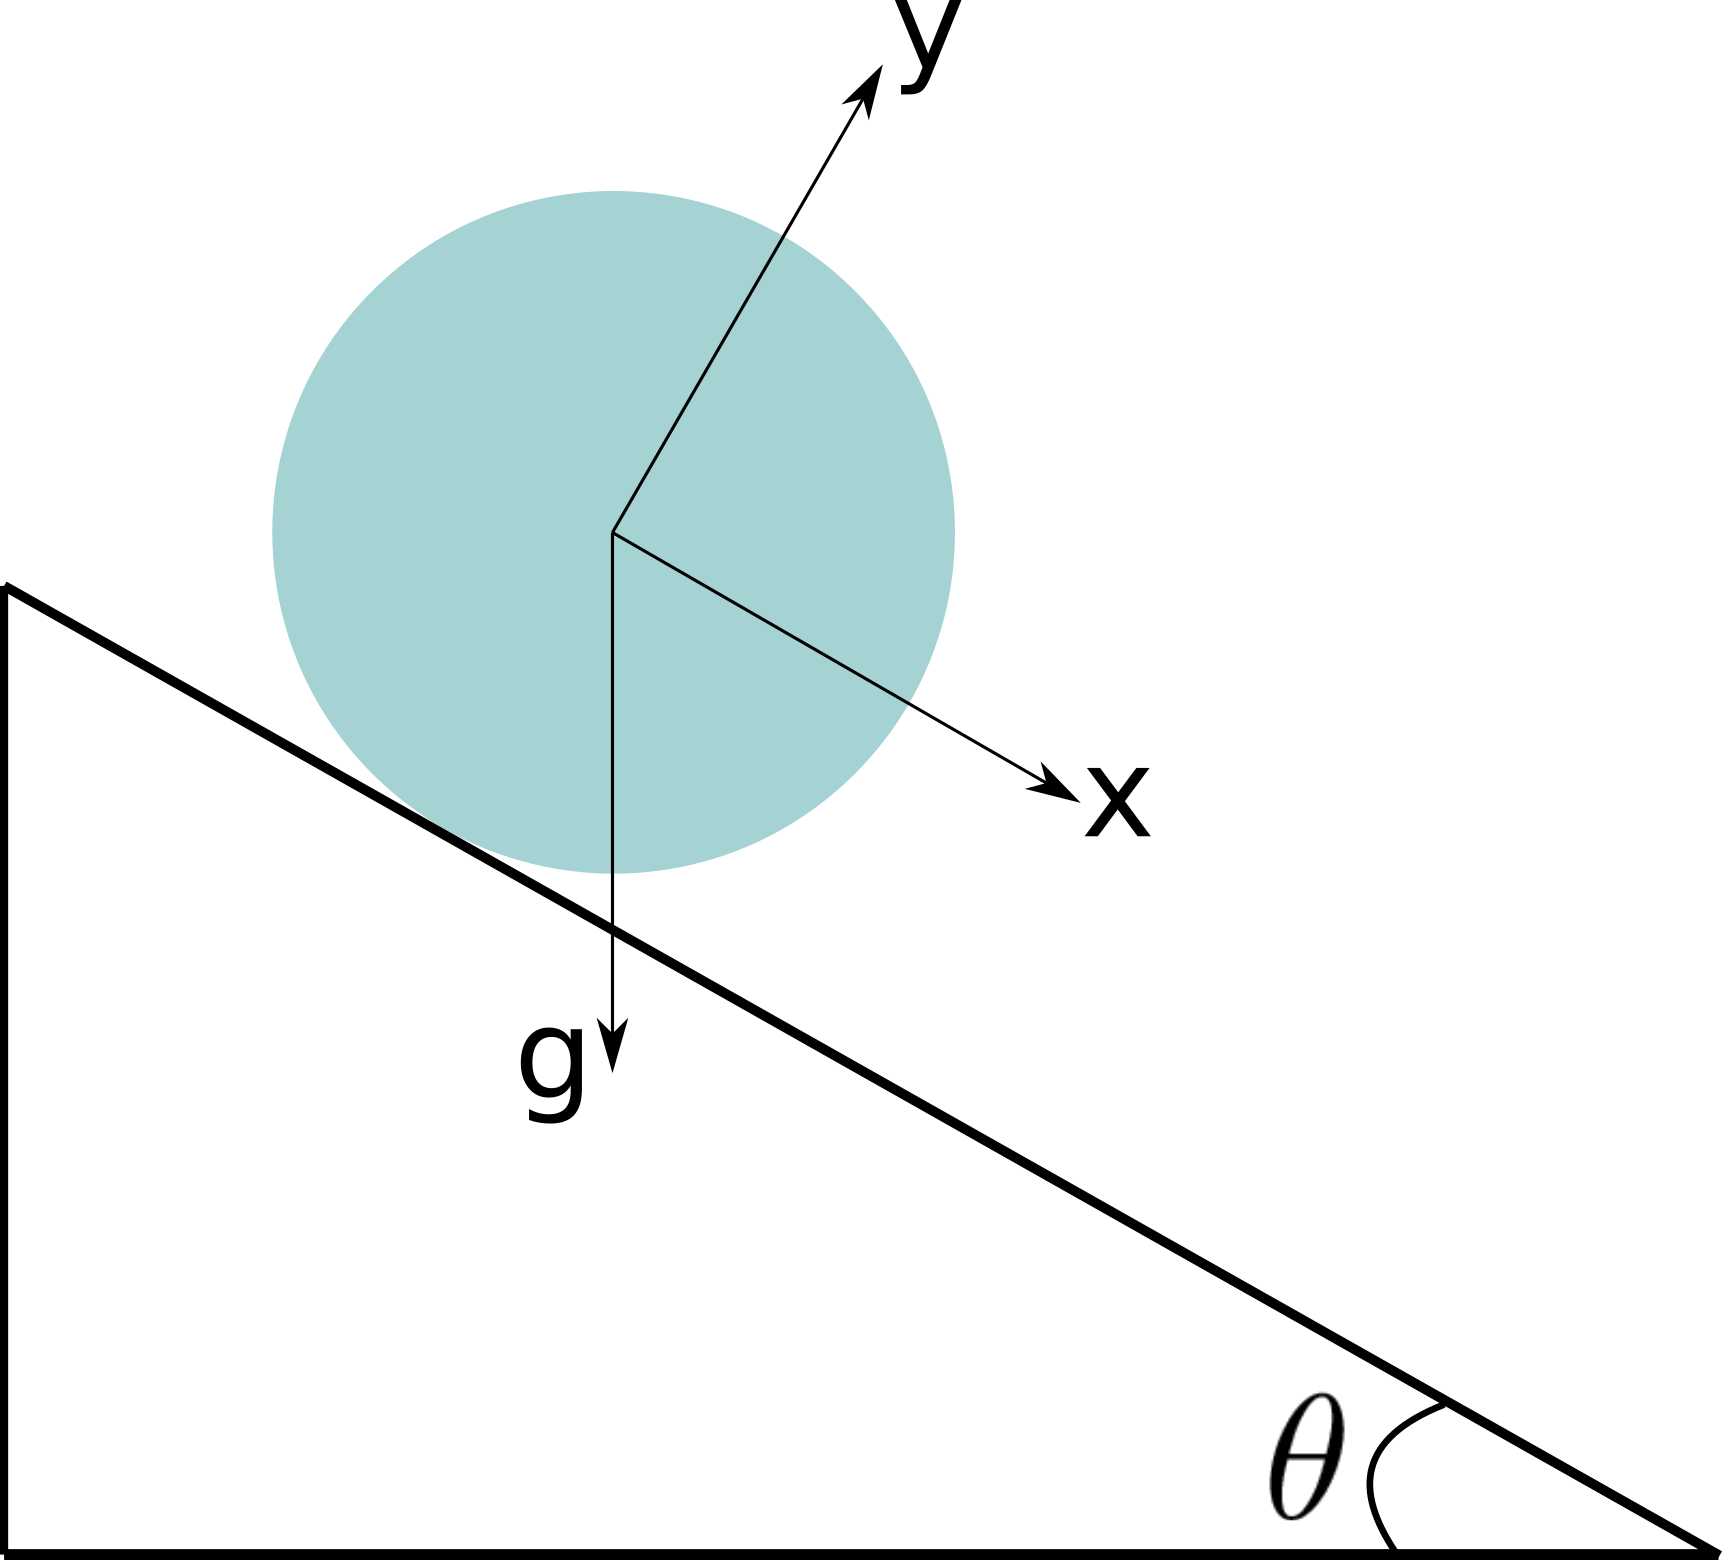
\includegraphics[width=1.0\textwidth]{images/de_2021_cylinder_rolling_on_an_inclined_plane/schematic_1}
%     \subcaption{}\label{fig:circular-body:schematic-1}
%   \end{subfigure}
%   \begin{subfigure}{0.48\textwidth}
%     \centering
%     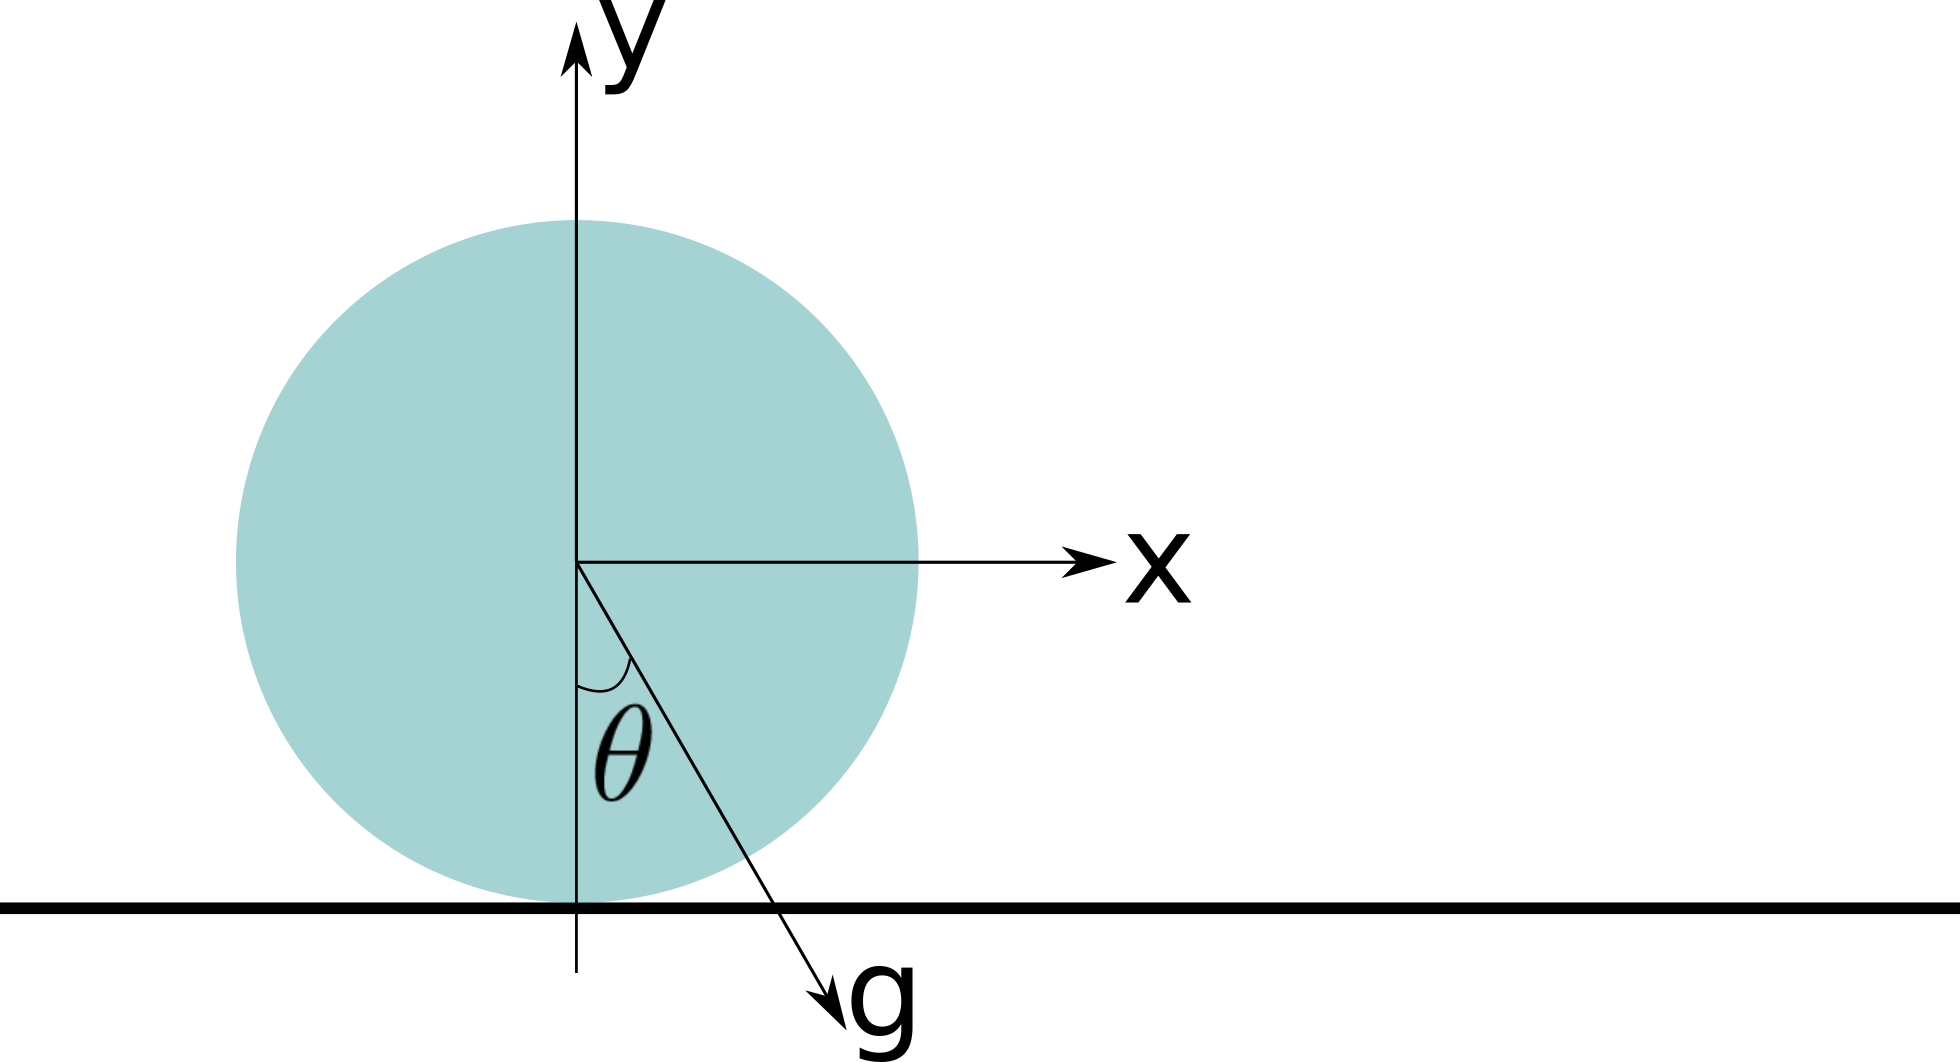
\includegraphics[width=1.0\textwidth]{images/de_2021_cylinder_rolling_on_an_inclined_plane/schematic_2}
%     \subcaption{}\label{fig:circular-body:schematic-2}
%   \end{subfigure}
%   \caption{A (a) physical and (b) computational model of the rolling cylinder on a
%     plane inclined at an angle $\theta$.}
% \label{fig:circular-body-schematic}
% \end{figure}
% \begin{table}[!ht]
%   \centering
%   \begin{tabular}[!ht]{ll}
%     \toprule
%     Quantity & Values\\
%     \midrule
%     $\rho$, density & $2700$ kg\,m\textsuperscript{-3} \\
%     $\mu$, friction coefficient & $0.3$ \& $0.6$ \\
%     Time of simulation & $0.6$ s \\
%     Resolution, $\delta x$ & $0.0025$ m\\
%     Smoothing length factor, $h/\Delta x$ & 1\\
%     gravity $[g_x, g_y, g_z]$ & $[g\,\sin(\theta), g\,\cos(\theta), 0.0]$\\
%     $k_r$, Repulsive stiffness coefficient & $1e7$ \\
%     $k_f$, Repulsive stiffness coefficient & $1e5$ \\
%     $\alpha_{damp}$ & 0.\\
%     \bottomrule
%   \end{tabular}
%   \caption{Material properties and numerical parameters used for the rolling
%     of cylinder on an inclined surface.}%
%   \label{tab:circular-body-rolling-params}
% \end{table}

% \Cref{fig:cylinder-xcom-vs-time} depicts the variation of center of mass of
% the cylinder with time for friction coefficients $0.3$ and $0.6$,
% respectively. From the \cref{fig:cylinder-xcom-vs-time} we can see that the
% current solver matches well with the analytical solution.
% \begin{figure}[!htpb]
%   \centering
%   \includegraphics[width=0.4\textwidth]{figures/de_2021_cylinder_rolling_on_an_inclined_plane_2d/xcom_vs_time}
%   \caption{x com vs time of a cylinder with a friction coefficient of $0.3$.}
% \label{fig:cylinder-xcom-vs-time}
% \end{figure}


% \FloatBarrier%
% \subsection{Rigid body sliding down an inclined plane}
% \label{sec:rigid-body-sliding}

% In the test case, we model free sliding of a rigid cube on an inclined plane.
% The frictional part of the current solver is validated through this test. The
% velocity of the center of mass of the cube is compared against the analytical
% solution for quantitative validation. The schematic is shown is
% \cref{fig:rigid_body_sliding}.
% \begin{figure}[!htpb]
%   \centering
%   \includegraphics[width=0.3\textwidth]{images/rigid_body_sliding/schematic}
%   \caption{}
% \label{fig:rigid_body_sliding}
% \end{figure}
% The rigid body of length $0.1$ m, height $0.1$, is allowed to slide on a
% frictional surface which is at an angle $\frac{\pi}{3}$. A density of $2000$
% kg\,m\textsuperscript{-3} is used for the body. Other numerical parameters,
% such as the repulsive spring stiffness $k_r=3.0 \times 10^{5}$ and tangential
% spring stiffness $k_t=3.0 \times 10^{5}$ is chosen, respectively. A particle
% spacing of $0.001$ is considered, resulting in $120$ particles in rigid body
% discretization. From the analytical solution, the evolution of velocity is
% given by,
% \begin{equation}
%   \label{eq:ce}
%   \ten{v}(t) = (\mu \teng{g} \sin (\theta) - \teng{g} \cos (\theta)) t.
% \end{equation}

% We have considered three different friction coefficients, $\mu=0.2$,
% $\mu=0.3$, and $\mu=0.6$. From the analytical solution, when the friction
% coefficient is greater than $\tan(frac{\pi}{3})$, we have no slip condition
% and the body doesn't slide.

% % \subsubsection{2D sliding}
% % \label{sec:results-2d-sliding}
% \Cref{fig:mohseni-2021-sliding-2d} shows the snapshots of the rigid body at
% three time instants. From \cref{fig:mohseni-2021-sliding-2d} we can see that
% the the body is freely sliding with out having any oscillations or unphysical
% jumping off the inclined wall. This is because of the new surface aware
% contact model as force is not computed by considering the wall as spherical
% \begin{figure}[!htpb]
%   \centering
%   \begin{subfigure}{0.48\textwidth}
%     \centering
%     \includegraphics[width=1.0\textwidth]{figures/mohseni_2021_free_sliding_on_a_slope_2d/fric_coeff_0_2/time0}
%     \subcaption{t = $0$ s}\label{fig:passing-0}
%   \end{subfigure}
%   %
%   \begin{subfigure}{0.48\textwidth}
%     \centering
%     \includegraphics[width=1.0\textwidth]{figures/mohseni_2021_free_sliding_on_a_slope_2d/fric_coeff_0_2/time1}
%     \subcaption{t = $0.5$ s}\label{fig:passing-1}
%   \end{subfigure}

%   \begin{subfigure}{0.48\textwidth}
%     \centering
%     \includegraphics[width=1.0\textwidth]{figures/mohseni_2021_free_sliding_on_a_slope_2d/fric_coeff_0_2/time2}
%     \subcaption{t = $1$ s}\label{fig:passing-2}
%   \end{subfigure}
%   \caption{Rigid body with friction $0.2$ sliding.}
% \label{fig:mohseni-2021-sliding-2d}
% \end{figure}
% particles but by ensemble of an overlap. The snapshots correspond to a
% friction coefficient of $0.2$.
% \Cref{fig:results-solid-sliding-velocity-vs-time-2d} shows a evolution of
% velocity of the center of mass of the rigid body for different frictional
% coefficients against the analytical solution. From
% \Cref{fig:results-solid-sliding-velocity-vs-time-2d} we can see that the current
% solver has an excellent match with the analytical solution and covers all the
% regimes of the sliding case.
% \begin{figure}[!htpb]
%   \centering
%   \includegraphics[width=0.4\textwidth]{figures/mohseni_2021_free_sliding_on_a_slope_2d/velocity_vs_time}
%   \caption{Velocity versus time}
% \label{fig:results-solid-sliding-velocity-vs-time-2d}
% \end{figure}

% % \subsubsection{3D sliding}
% % \label{sec:results-3d-sliding}

% % \Cref{fig:mohseni-2021-sliding-3d} shows the snapshots of the rigid body at 4
% % time instants. From \cref{fig:mohseni-2021-sliding-3d} we can see that the the
% % body is freely sliding with out having any oscillations or unphysical jumping
% % off the inclined wall. This is because of the new surface aware contact model
% % as force is not computed by considering the wall as spherical particles but by
% % ensemble of an overlap. The snapshots correspond to a friction coefficient of
% % $0.4$. \Cref{fig:results-solid-sliding-velocity-vs-time-3d} shows a evolution of
% % velocity of the center of mass of the rigid body for different frictional
% % coefficients against the analytical solution. From
% % \Cref{fig:results-solid-sliding-velocity-vs-time-3d} we can see that the current
% % solver has an excellent match with the analytical solution and covers all the
% % regimes of the sliding case.
% % \begin{figure}[!htpb]
% %   \centering
% %   \includegraphics[width=0.6\textwidth]{figures/mohseni_2021_free_sliding_on_a_slope_3d/velocity_vs_time}
% %   \caption{Velocity versus time}
% % \label{fig:results-solid-sliding-velocity-vs-time-3d}
% % \end{figure}

% % \begin{figure}[!htpb]
% %   \centering
% %   \begin{subfigure}{0.48\textwidth}
% %     \centering
% %     \includegraphics[width=1.0\textwidth]{figures/mohseni_2021_free_sliding_on_a_slope_3d/fric_coeff_0_2/time0}
% %     \subcaption{t = 2.5e-03 sec}\label{fig:passing-0}
% %   \end{subfigure}
% %   %
% %   \begin{subfigure}{0.48\textwidth}
% %     \centering
% %     \includegraphics[width=1.0\textwidth]{figures/mohseni_2021_free_sliding_on_a_slope_3d/fric_coeff_0_2/time1}
% %     \subcaption{t = 2.5e-03 sec}\label{fig:passing-1}
% %   \end{subfigure}

% %   \begin{subfigure}{0.48\textwidth}
% %     \centering
% %     \includegraphics[width=1.0\textwidth]{figures/mohseni_2021_free_sliding_on_a_slope_3d/fric_coeff_0_2/time2}
% %     \subcaption{t = 2.5e-03 sec}\label{fig:passing-2}
% %   \end{subfigure}
% %   \caption{Rigid body with friction $0.2$ sliding.}
% % \label{fig:mohseni-2021-sliding-3d}
% % \end{figure}


% \FloatBarrier%
% \subsection{Controlled Sliding on a Flat Surface}
% \label{sec:controlled-rigid-body-sliding}
% A rigid body to slide on a frictional flat surface by applying an external
% normal $F$ and tangential force $F$. The friction coefficient between the
% body and wall is assumed to be $0.5$. The schematic of the rigid body as well
% as the wall is shown in \cref{fig:schematic-controlled-rigid-body-sliding}.
% \begin{figure}[!htpb]
%   \centering
%   \includegraphics[width=0.3\textwidth]{images/controlled_rigid_body_sliding/schematic}
%   \caption{Schematic of the controlled rigid body sliding}
% \label{fig:schematic-controlled-rigid-body-sliding}
% \end{figure}
% The force $\bold{F}$ is applied on top of the body for a time of $1.5$
% seconds, which gradually increases to $2000$ N till time $0.5$ seconds, and
% stays constant till time $1.5$ seconds. Once the normal force $bold{N}$
% reaches $2000$ N, we start applying the tangential force and increase it to
% $4000$ N till time $1.0$ seconds. These force variation is shown in
% \cref{fig:velocity-vs-time-controlled-sliding}.

% \Cref{fig:velocity-vs-time-controlled-sliding} depicts the time histories of
% velocity of the center of mass of the rigid body with time, as well as the
% variation of applied external normal $\bold{F}$ and tangential $\bold{T}$
% forces against the velocity computed using analytical solution.
% \begin{figure}[!htpb]
%   \centering
%   \includegraphics[width=0.7\textwidth]{figures/mohseni_2021_controlled_sliding_on_a_flat_surface_2d/case_1/force_velocity_vs_t}
%   \caption{Velocity vs time of the rigid slider}
% \label{fig:velocity-vs-time-controlled-sliding}
% \end{figure}


% % \FloatBarrier
% % \subsection{Three bodies colliding}
% % \label{sec:three-bodies-colliding}


% % \begin{figure}[!htpb]
% %   \centering
% %   % \includegraphics[width=0.4\textwidth]{figures/mohseni_2021_free_sliding_on_a_slope_3d/velocity_vs_time}
% %   \caption{Schematic of the three rigid body colliding}
% % \label{fig:schematic-three-rigid-bodies-colliding}
% % \end{figure}

% % \begin{figure}[!htpb]
% %   \centering
% %   \begin{subfigure}{0.48\textwidth}
% %     \centering
% %     \includegraphics[width=1.0\textwidth]{figures/amaro_2019_collision_between_three_rigid_cubes/Mohseni_Vyas/time0}
% %   \end{subfigure}
% %   %
% %   \begin{subfigure}{0.48\textwidth}
% %     \centering
% %     \includegraphics[width=1.0\textwidth]{figures/amaro_2019_collision_between_three_rigid_cubes/Mohseni_Vyas/time1}
% %   \end{subfigure}

% %   \begin{subfigure}{0.48\textwidth}
% %     \centering
% %     \includegraphics[width=1.0\textwidth]{figures/amaro_2019_collision_between_three_rigid_cubes/Mohseni_Vyas/time2}
% %   \end{subfigure}
% %   %
% %   \begin{subfigure}{0.48\textwidth}
% %     \centering
% %     \includegraphics[width=1.0\textwidth]{figures/amaro_2019_collision_between_three_rigid_cubes/Mohseni_Vyas/time3}
% %   \end{subfigure}
% % \caption{A dummy figure (To be fixed)}
% % \label{fig:snapshots-three-cubes-colliding}
% % \end{figure}
% % %


% \FloatBarrier%
% \subsection{Stack of cylinders}
% \label{sec:stack-of-cylinders}

% This test case is used to validate the current solid-solid contact force
% model. A stack of cylinders initially at rest are allowed to settle under
% gravity in a tank. This is simulated by Zhang (2011), where DEM is used. The
% numerical parameters of the current test case are listed in
% \Cref{tab:stack-of-cylinders}. The dimensions of the cylinder as well as the
% tank are shown in figure (Ref the schematic figure).

% \begin{table}[!ht]
%   \centering
%   \begin{tabular}[!ht]{ll}
%     \toprule
%     Quantity & Values\\
%     \midrule
%     $L$, length of the domain & 1 m \\
%     Time of simulation & 2.5 s \\
%     $c_s$ & 10 m/s \\
%     $\rho_0$, reference density & 1 kg/m\textsuperscript{3} \\
%     Reynolds number & 200 \& 1000 \\
%     Resolution, $L/\Delta x_{\max} : L/\Delta x_{\min}$ & $[100:200]$ \& $[150:300]$\\
%     Smoothing length factor, $h/\Delta x$ & 1.0\\
%     \bottomrule
%   \end{tabular}
%   \caption{Parameters used for the Taylor-Green vortex problem.}%
%   \label{tab:stack-of-cylinders}
% \end{table}

% \Cref{fig:snapshots-stack-of-cylinders} presents a set of snapshots
% corresponding to the simulation of a stack of cylinders collapsing under
% gravity using CTVF-DEM in comparison with the corresponding experimental
% photos by Zhang. From the presented figure, the reproduced cylinder's
% positions appear to be consistent with those observed in the experiment. From
% \Cref{fig:snapshots-stack-of-cylinders}, the current solver has presented
% proper level of stability.

% \begin{figure}[!htpb]
%   \centering
%   \begin{subfigure}{0.48\textwidth}
%     \centering
%     \includegraphics[width=1.0\textwidth]{figures/stack_of_cylinders_2d/Mohseni_Vyas/time0}
%   \end{subfigure}
%   %
%   \begin{subfigure}{0.48\textwidth}
%     \centering
%     \includegraphics[width=0.75\textwidth]{images/stack_of_cylinders_experimental_images/time0}
%   \end{subfigure}

%   \begin{subfigure}{0.48\textwidth}
%     \centering
%     \includegraphics[width=1.0\textwidth]{figures/stack_of_cylinders_2d/Mohseni_Vyas/time1}
%   \end{subfigure}
%   %
%   \begin{subfigure}{0.48\textwidth}
%     \centering
%     \includegraphics[width=0.75\textwidth]{images/stack_of_cylinders_experimental_images/time1}
%   \end{subfigure}

%   \begin{subfigure}{0.48\textwidth}
%     \centering
%     \includegraphics[width=1.0\textwidth]{figures/stack_of_cylinders_2d/Mohseni_Vyas/time2}
%   \end{subfigure}
%   %
%   \begin{subfigure}{0.48\textwidth}
%     \centering
%     \includegraphics[width=0.75\textwidth]{images/stack_of_cylinders_experimental_images/time2}
%   \end{subfigure}

%   \begin{subfigure}{0.48\textwidth}
%     \centering
%     \includegraphics[width=1.0\textwidth]{figures/stack_of_cylinders_2d/Mohseni_Vyas/time3}
%   \end{subfigure}
%   %
%   \begin{subfigure}{0.48\textwidth}
%     \centering
%     \includegraphics[width=0.75\textwidth]{images/stack_of_cylinders_experimental_images/time3}
%   \end{subfigure}
% \caption{A dummy figure (To be fixed)}
% \label{fig:snapshots-stack-of-cylinders}
% \end{figure}
% %


% \Cref{fig:x-com-stack-of-cylinders,fig:y-com-stack-of-cylinders} presents the
% time histories of the x and y components of the center of mass of the
% cylinders respectively as well as those from numerical simulations by
% SPH-DCDEM as well as MPS-DEM with respect to those from the experiment Zhang.
% From the presented figure, the effective center of mass of the cylinders is in
% good agreement with the experiment.

% \begin{figure}[!htpb]
%   \centering
%   \includegraphics[width=0.4\textwidth]{figures/stack_of_cylinders_2d/Mohseni_Vyas/xcom}
%   \caption{A dummy figure (To be fixed)}
% \label{fig:x-com-stack-of-cylinders}
% \end{figure}
% \begin{figure}[!htpb]
%   \centering
%   \includegraphics[width=0.4\textwidth]{figures/stack_of_cylinders_2d/Mohseni_Vyas/ycom}
%   \caption{A dummy figure (To be fixed)}
% \label{fig:y-com-stack-of-cylinders}
% \end{figure}


% \FloatBarrier%
% \subsection{Falling solid in water}
% \label{sec:falling-solid-in-water}

% In this section, the rigid fluid coupling part of the current solver is
% evaluated by simulation of a rigid cube falling in an hydrostatic tank (cite
% experimental paper). The CTVF-DEM solver is employed to simulate water entry
% of a rigid cube, which is studied experimentally by (cite the paper). The
% numerical parameters of the current test case are listed in
% \Cref{tab:stack-of-cylinders}. The dimensions of the schematic are shown in
% figure.

% \begin{table}[!ht]
%   \centering
%   \begin{tabular}[!ht]{ll}
%     \toprule
%     Quantity & Values\\
%     \midrule
%     $L$, length of the domain & 1 m \\
%     Time of simulation & 2.5 s \\
%     $c_s$ & 10 m/s \\
%     $\rho_0$, reference density & 1 kg/m\textsuperscript{3} \\
%     Reynolds number & 200 \& 1000 \\
%     Resolution, $L/\Delta x_{\max} : L/\Delta x_{\min}$ & $[100:200]$ \& $[150:300]$\\
%     Smoothing length factor, $h/\Delta x$ & 1.0\\
%     \bottomrule
%   \end{tabular}
%   \caption{Parameters used for the Taylor-Green vortex problem.}%
%   \label{tab:stack-of-cylinders}
% \end{table}

% A rigid cube of a side length of 30 mm enters the water initially at
% hydrostatic state with a velocity of 30 $m/s$ in z-direction.
% \Cref{fig:snapshots-falling-solid-in-water} presents a snapshots of the rigid
% cube falling in an hydrostatic tank with the current solver as well as
% WCSPH-DEM solver as well as the experimental result. From the presented figure
% \Cref{fig:snapshots-falling-solid-in-water}, we can see that the pressure
% distribution is smooth and the simulation is stable. A zoomed in view near the
% rigid cube is presented in \cref{fig:snapshots-falling-solid-in-water-zoomed}
% when simulated with WCSPH-DEM and CTVF-DEM. From
% \cref{fig:snapshots-falling-solid-in-water-zoomed} we can see that the fluid
% particle distribution around the body with CTVF scheme is uniform when
% compared with WCSPH, thanks to the implemented transport velocity formulation.

% \begin{figure}[!htpb]
%   \centering
%   \begin{subfigure}{0.48\textwidth}
%     \centering
%     \includegraphics[width=1.0\textwidth]{figures/qiu_2017_falling_solid_in_water_2d/dx_0_002/time0}
%   \end{subfigure}
%   %
%   \begin{subfigure}{0.48\textwidth}
%     \centering
%     \includegraphics[width=1.0\textwidth]{figures/qiu_2017_falling_solid_in_water_2d/dx_0_002/time1}
%   \end{subfigure}

%   \begin{subfigure}{0.48\textwidth}
%     \centering
%     \includegraphics[width=1.0\textwidth]{figures/qiu_2017_falling_solid_in_water_2d/dx_0_002/time2}
%   \end{subfigure}
%   %
%   \begin{subfigure}{0.48\textwidth}
%     \centering
%     \includegraphics[width=1.0\textwidth]{figures/qiu_2017_falling_solid_in_water_2d/dx_0_002/time3}
%   \end{subfigure}
% \caption{A dummy figure (To be fixed)}
% \label{fig:snapshots-falling-solid-in-water}
% \end{figure}

% \begin{figure}[!htpb]
%   \centering
%   \begin{subfigure}{0.48\textwidth}
%     \centering
%     \includegraphics[width=1.0\textwidth]{figures/qiu_2017_falling_solid_in_water_2d/dx_0_002/time0}
%   \end{subfigure}
%   %
%   \begin{subfigure}{0.48\textwidth}
%     \centering
%     \includegraphics[width=1.0\textwidth]{figures/qiu_2017_falling_solid_in_water_2d/dx_0_002/time1}
%   \end{subfigure}

%   \begin{subfigure}{0.48\textwidth}
%     \centering
%     \includegraphics[width=1.0\textwidth]{figures/qiu_2017_falling_solid_in_water_2d/dx_0_002/time2}
%   \end{subfigure}
%   %
%   \begin{subfigure}{0.48\textwidth}
%     \centering
%     \includegraphics[width=1.0\textwidth]{figures/qiu_2017_falling_solid_in_water_2d/dx_0_002/time3}
%   \end{subfigure}
%   \caption{Zoomed in snapshots of rigid body inside water.}
% \label{fig:snapshots-falling-solid-in-water-zoomed}
% \end{figure}

% \Cref{fig:disp-falling-solid-in-water} presents the time history of the
% displacement of the rigid cube with time in comparison with the experimental
% result by (cite experimental paper). From the presented figure, the CTVF-DEM
% model has reproduced the displacement of the rigid cube with acceptable levels
% of stability as well as accuracy.
% \begin{figure}[!htpb]
%   \centering
%   \includegraphics[width=0.4\textwidth]{figures/qiu_2017_falling_solid_in_water_2d/y_cm_vs_time}
%   \caption{Center of mass of rigid body vs time compared with experiment}
% \label{fig:disp-falling-solid-in-water}
% \end{figure}


% \FloatBarrier%
% \subsection{Floating solid in water, 500 density cube}
% \label{sec:floating-solid-in-water}

% To be done



% % \FloatBarrier%
% % \subsection{A rigid box rotating and sinking in viscous liquid}
% % Rotating box in fluid \cite{sun2015numerical}.


% % \FloatBarrier%
% % \subsection{Water entry of 2-D cylinder}
% % Water entry of 2-D cylinder \cite{sun2015numerical}.


% % \FloatBarrier%
% % \subsection{2d wedge entry in water}
% % \label{sec:wedge-entry-in-water}

% % To be done

% \FloatBarrier%
% \subsection{Water-entry of a single sphere}
% \label{sec:water-entry-sphere}
% % https://www.sciencedirect.com/science/article/pii/S0997754621001412#fig2

% In this section we reproduce the water entry of a single sphere experiment
% done by \cite{aristoff_water_2010}. A sphere of diameter $24.4$ mm is allowed
% to settle under gravity in a water tank of dimensions, $0.2$ m $\times$ $0.2$
% m $\times$ $0.14$ m, with a water depth of $0.11$ m
% (\cref{fig:water-entry-sphere-schematic}). The initial velocity of the sphere
% is $2.17$ m/s. A convergence study of the current rigid fluid coupling
% algorithm is carried out by simulating a total of 3 resolution studies ($0.01$
% m, $0.005$ m, $0.002$ m) is carried out.

% \begin{figure}[!htpb]
%   \centering
%   \includegraphics[width=0.4\textwidth]{images/water_entry_of_sphere/schematic}
%   \caption{Schematic}
% \label{fig:water-entry-sphere-schematic}
% \end{figure}



% \FloatBarrier%
% \subsection{Settling of two identical cylinders in series}
% \label{sec:water-entry-sphere}
% % https://www.sciencedirect.com/science/article/pii/S0997754621001412#fig2

% In this section we reproduce the water entry of a single sphere experiment
% done by \cite{aristoff_water_2010}. A sphere of diameter $24.4$ mm is allowed
% to settle under gravity in a water tank of dimensions, $0.2$ m $\times$ $0.2$
% m $\times$ $0.14$ m, with a water depth of $0.11$ m
% (\cref{fig:cylinders-in-series-schematic}). The initial velocity of the sphere
% is $2.17$ m/s. A convergence study of the current rigid fluid coupling
% algorithm is carried out by simulating a total of 3 resolution studies ($0.01$
% m, $0.005$ m, $0.002$ m) is carried out.
% \begin{figure}[!htpb]
%   \centering
%   \includegraphics[width=0.4\textwidth]{images/two_cylinders_one_top_of_another/schematic}
%   \caption{Schematic}
% \label{fig:cylinders-in-series-schematic}
% \end{figure}


% % \FloatBarrier%
% % \subsection{Two identical spheres settlement side by side}
% % \label{sec:water-entry-sphere}
% % % https://www.sciencedirect.com/science/article/pii/S0997754621001412#fig2

% % In this test we study the behaviour of two spheres setting inside a fluid
% % tank. This test comprises of complex rigid-fluid coupling phenomena as well as
% % the rigid interaction between the spheres. The dimensions of the sphere and
% % % the fluid including the tank are shown in \cref{}.

% % The initial velocity of the sphere is $2.17$ m/s. A convergence
% % study of the current rigid fluid coupling algorithm is carried out by
% % simulating a total of 3 resolution studies ($0.01$ m, $0.005$ m, $0.002$ m) is
% % carried out.


% \FloatBarrier%
% \subsection{3D dam breaking flow hitting cubes}

% \cite{amaro2019improvement}

% In the current case we simulate a 3d dam breaking flow hitting different
% configuration of rigid cubes. This is experimentally studied by SPH DCDEM,
% where the author used Direct Linear Transform (DLT) to track the cubes as they
% move after the impact. A total three rigid body configurations are studied, a
% single cube, three cubes and a pyramid configuration, respectively. It is
% numerically studied by SPH-DCDEM, MPS-DEM, and (cite some other papers). The
% side length of each cube is $3.5$ mm and the material properties are listed in
% \cref{tab:material-properties-3d-dam-breaking-flow-hitting-cubes} and the
% numerical parameters are given in
% \cref{tab:material-properties-3d-dam-breaking-flow-hitting-cubes}. In all the
% three cases the fluid is initially allowed to flow by opening a gate which
% lifts at a velocity of 3.5 m\,s\textsuperscript{-1}

% \begin{table}[!ht]
%   \centering
%   \begin{tabular}[!ht]{ll}
%     \toprule
%     Quantity & Values\\
%     \midrule
%     $L$, length of the domain & 1 m \\
%     $\rho_0$, reference density & 1 kg/m\textsuperscript{3} \\
%     Reynolds number & 200 \& 1000 \\
%     Resolution, $L/\Delta x_{\max} : L/\Delta x_{\min}$ & $[100:200]$ \& $[150:300]$\\
%     \bottomrule
%   \end{tabular}
%   \caption{Parameters used for the Taylor-Green vortex problem.}%
%   \label{tab:material-properties-3d-dam-breaking-flow-hitting-cubes}
% \end{table}

% \begin{table}[!ht]
%   \centering
%   \begin{tabular}[!ht]{ll}
%     \toprule
%     Quantity & Values\\
%     \midrule
%     $L$, length of the domain & 1 m \\
%     $\rho_0$, reference density & 1 kg/m\textsuperscript{3} \\
%     Reynolds number & 200 \& 1000 \\
%     Resolution, $L/\Delta x_{\max} : L/\Delta x_{\min}$ & $[100:200]$ \& $[150:300]$\\
%     \bottomrule
%   \end{tabular}
%   \caption{Parameters used for the Taylor-Green vortex problem.}%
%   \label{tab:numerical-properties-3d-dam-breaking-flow-hitting-cubes}
% \end{table}

% \Cref{fig:snapshots-single-cube-3d-dam-breaking-flow} shows the snapshots of
% the rigid cube moving downstream of the tank when interacting with the fluid
% flow against the experimental result (cite SPH DCDEM). From
% \Cref{fig:snapshots-single-cube-3d-dam-breaking-flow} we can see that the
% rigid cube matches well with the experimental result. Further, we compare the
% positions of the rigid cube with time in
% \Cref{fig:x-position-single-cube-3d-dam-breaking-flow}, against the
% experimental results, SPH-DCDEM, MPS-DEM results. It can be seen from figure
% \Cref{fig:x-position-single-cube-3d-dam-breaking-flow} that the current solver
% is able to provide good accuracy in producing the correct displacement of the
% cube and agrees well with the experimental as well as the other numerical
% techniques.
% \begin{figure}[!htpb]
%   \centering
%   \includegraphics[width=0.4\textwidth]{figures/mohseni_2021_free_sliding_on_a_slope_3d/velocity_vs_time}
%   \caption{Snapshots of a single cube under a 3d dam breaking flow}
% \label{fig:snapshots-single-cube-3d-dam-breaking-flow}
% \end{figure}
% \begin{figure}[!htpb]
%   \centering
%   \includegraphics[width=0.4\textwidth]{figures/amaro_2019_dam_breaking_flow_hitting_one_cube_3d/case_1/xcom_vs_time}
%   \caption{x position of the cube with time for single cube.}
% \label{fig:x-position-single-cube-3d-dam-breaking-flow}
% \end{figure}

% The initial configuration of the dam breaking flow over three cubes is shown
% in figure \Cref{fig:snapshots-three-cubes-3d-dam-breaking-flow}.
% \Cref{fig:snapshots-three-cubes-3d-dam-breaking-flow} shows the snapshots of
% the rigid cubes at different time instants from the start of fluid hit with
% the color of the fluid particles representing pressure. From the
% \Cref{fig:snapshots-three-cubes-3d-dam-breaking-flow} we can see that the
% simulated rigid bodies match well with the experimental observations. We also
% compare the x component of the effective center of mass of the three cubes
% with time in \Cref{fig:x-position-three-cubes-3d-dam-breaking-flow}, against
% the experimental results, SPH-DCDEM, MPS-DEM results. From figure
% \Cref{fig:x-position-three-cubes-3d-dam-breaking-flow}, we can see that the
% current solve is agrees well with the experimental as well as with the other
% numerical method results.
% \begin{itemize}
% \item Mention at what time does the fluid hits the rigid cubes.
% \end{itemize}
% \begin{figure}[!htpb]
%   \centering
%   \includegraphics[width=0.4\textwidth]{figures/mohseni_2021_free_sliding_on_a_slope_3d/velocity_vs_time}
%   \caption{Snapshots of a three cubes under a 3d dam breaking flow}
% \label{fig:snapshots-three-cubes-3d-dam-breaking-flow}
% \end{figure}
% \begin{figure}[!htpb]
%   \centering
%   \includegraphics[width=0.4\textwidth]{figures/amaro_2019_dam_breaking_flow_hitting_three_stacked_cubes_3d/case_1/xcom_vs_time}
%   \caption{x position of the cubes with time for three cube.}
% \label{fig:x-position-three-cubes-3d-dam-breaking-flow}
% \end{figure}
% \begin{figure}[!htpb]
%   \centering
%   \includegraphics[width=0.4\textwidth]{figures/amaro_2019_dam_breaking_flow_hitting_three_stacked_cubes_3d/case_1/ycom_vs_time}
%   \caption{y position of the cubes with time for three cube.}
% \label{fig:y-position-three-cubes-3d-dam-breaking-flow}
% \end{figure}


% The placement of the cubes in the pyramid configuration including dimensions,
% distance from the left wall and other dimension related information can be
% seen in figure \Cref{fig:snapshots-three-cubes-3d-dam-breaking-flow}.
% \Cref{fig:snapshots-three-cubes-3d-dam-breaking-flow} shows the snapshots of
% the rigid cubes at different time instants and the color coding of the fluid
% particles represents pressure. From
% \Cref{fig:snapshots-three-cubes-3d-dam-breaking-flow}, it can be seen that the
% rigid body positions are in match with the experimental observations. Which is
% further validated by doing a quantitative comparison of the x component of
% effective center of mass of the six cubes in time against the experimental
% results, SPH-DCDEM, MPS-DEM results in
% \Cref{fig:x-position-six-cubes-3d-dam-breaking-flow}. From these figures, we
% can see that the current solver is in good agreement with the other numerical
% and experimental results.
% \begin{figure}[!htpb]
%   \centering
%   \includegraphics[width=0.4\textwidth]{figures/mohseni_2021_free_sliding_on_a_slope_3d/velocity_vs_time}
%   \caption{Snapshots of six cubes under a 3d dam breaking flow}
% \label{fig:snapshots-six-cubes-3d-dam-breaking-flow}
% \end{figure}
% \begin{figure}[!htpb]
%   \centering
%   \includegraphics[width=0.4\textwidth]{figures/amaro_2019_dam_breaking_flow_hitting_six_stacked_cubes_3d/case_1/xcom_vs_time}
%   \caption{x position of the cubes with time for six cubes.}
% \label{fig:x-position-six-cubes-3d-dam-breaking-flow}
% \end{figure}
% \begin{figure}[!htpb]
%   \centering
%   \includegraphics[width=0.4\textwidth]{figures/amaro_2019_dam_breaking_flow_hitting_six_stacked_cubes_3d/case_1/ycom_vs_time}
%   \caption{y position of the cubes with time for six cubes.}
% \label{fig:y-position-six-cubes-3d-dam-breaking-flow}
% \end{figure}


% \subsection{Dam break with body transport}
% \label{sec:dam-break-with-body-transport}

% \citet{wang2019numerical}

% \subsection{Dam break with multiple bodies transport}
% \label{sec:dam-break-with-multiple-bodies-transport}
% \citet{wang2019numerical}


% \subsection{Cylinders in water collapsed under gravity}
% \label{sec:cylinders-collapse-in-water}
% \citet{chen2019coupled}


% \section{Conclusions}
% \label{sec:conclusions}

% In this paper we coupled CTVF and DEM to simulate a two-way rigid-fluid coupling
% phenomenon. The fluid phase is handled by the CTVF scheme, whereas a modified
% contact force formulation is used to handle the interaction between the
% arbitrarily shaped rigid bodies.

% It has been demonstrated that the current model is able to predict the post
% collision behaviour of the colliding bodies by simulating collision between
% flat, and curved interfaces in two and three dimensions. A sliding elastic
% body is simulated to test the frictional part of the contact model. Finally,
% the full scale model is applied to model the stress propagation in granular
% discs for the first time in SPH. The results compare well with those of FEM as
% well as analytical studies.


% Further, we have made our implementation open-source.


% For future work, we plan to extend the current solver being extended to handle
% rigid fluid coupling in multiphase flows. Cavitation induced due to the entry
% of rigid objects can be studied. The particle-shifting strategy will be
% helpful in studying the occuring of cavitation due to rigid body entries.
% Further, the current work can be applied to study biomedical applications,
% such as red blood cells transport in a non-newtonian fluid flow, impact of
% arbitrarily shaped rigid objects in fluid flow to note a few.




\section*{References}


\bibliographystyle{model6-num-names}
\bibliography{references}


\end{document}
%%% Local Variables:
%%% mode: latex
%%% TeX-master: "paper"
%%% fill-column: 78
%%% End:



% \begin{enumerate}
% \item DOF
% \item Variables to describe the state
% \item Governing equations
% \item Discretization
% \item Two coordinate system (Particle positions about these two)
% \item Updated state
% \item Rotation matrix
% \item (a) Describe how the particles are translated to gloabl system from
%   local using rotation matrix. Use a figure.
% \item (b) Particle positions about new Rr
% \item $\omega$ and $\ten{R}$ relation
% \item Relation $I$ and $\ten{R}$
% \item Integration of governing equations
% \item Advantages of representing the body with just boundary particles and
%   speed up
% \end{enumerate}
